\begin{apendicesenv}
	\chapter{Como fazer uma rede neural}
	
	\section{Entendo aproximadores de função}
		\begin{itemize}
			\item Analisar o contexto do problema: O mesmo é linear, não linear \cite{rashid2016make}.
			\item A partir do item anterior, definir qual a função da ativação será usada \cite{rashid2016make}.
		\end{itemize}
	
		\par É importante também, dependendo do tipo de problema, saber escolher uma função de cálculo de erro, essa função, pode ser uma função quadrática, linear ou outra dependendo da importância que o erro tem na solução do problema. As funções de cálculo de erro mais usadas são mostradas abaixo:
		
		%TODO Colocar  exemplos de função de cálculo de erros
		\begin{itemize}
			\item $erro = valorDesejado - valorCalculado$
			\item 
		\end{itemize}
	
		\par Calculado o erro é necessário agora, de alguma forma, fazer com que esse erro seja corrigido utilizando uma abordagem iterativa que se aproxima cada vez mais do valor desejado usando pequenos passos. Considerando que $\Delta$ represente uma pequena variação em um valor $peso$, e sendo  $peso$ um dos parâmetros da função de ativação de um aproximador ($y = peso . x$ para uma função de ativação linear) então temos que a correção do valor deve ser dado como na equação abaixo:
		
		\begin{equation}
			valorDesejado = (peso + \Delta peso) . entrada \qquad,
		\end{equation}
		\cite{rashid2016make}
		
		\par Então, sabendo que o $valorDesejado = peso + \Delta peso . entrada$ e que $erro = valorDesejado - valorCalculado$ se pode concluir que:
		
		\begin{equation}
			\Delta peso = \dfrac{erro} { entrada} \qquad,
		\end{equation}
	
		\par No tocante as funções de ativação se pode imaginar quantas forem necessárias, no entanto, algumas se destacam dentro do campo das redes neurais:
	
		\begin{itemize}
			\item \textit{step function}: \begin{equation}
				y = \begin{cases} 
					0 & x\leq 0 \\
					1 & x > 0 \\
				\end{cases}
			\end{equation}
			\item \textit{sigmoid function}: \begin{equation}
				y = \dfrac{1}{1 + e^{-x}}
			\end{equation}
			%TODO Apresentar outro exemplos de função de ativação
		\end{itemize}
	
		\par No entanto, existe um problema quanto a esta abordagem, a função de ativação que recebe o parâmetro $peso$ Se adaptará ao último exemplo mostrado a ela criando uma situação conhecida como "overfitting", invalidando assim todos os os outros exemplos anteriormente usados, portanto, como se pode notar, é necessário a criação de um elemento que impeça esse ajustamento extremo, chamado de taxa de aprendizado:
		
		\begin{equation}
			\Delta peso = taxaDeAprendizado . \left( \dfrac{erro} { entrada} \right) \qquad,
		\end{equation}
			
		\par Usualmente a taxa de aprendizado é um valor suficientemente pequeno cujo o objetivo é garantir que o \textit{ovefitting} não aconteça mas, suficientemente grande para que a rede aprenda em um tempo razoável. Sendo $0,1$ um dos valores normalmente usados.
		%TODO Não citar redes neurais nessa sessão
	\section{Junção dos aproximadores: Redes neurais }
		\par Já que a sessão anterior definiu o que é um aproximador de funções, nesta sessão, usando as definições já vistas, será apresentada a definição de uma rede neural que é a junção de vários aproximadores que, dessa forma, conseguem  delimitar espaços de resultados mais complexos além daqueles que podem ser separados por apenas uma função de ativação.
		
		\par Um dos exemplos clássicos que necessitam dessa abordagem mais complexa é o exemplo da porta lógica \textit{xor}. Quando se tenta usar apenas um aproximador de funções para conseguir os resultados dessa porta é possível notar que o mesmo não é capaz de criar um espaço de resultados suficientemente complexo afim de separar os pontos fornecidos, sendo assim, Torna-se necessário o uso de múltiplos aproximadores (ou, nesse caso, 2).
		
		\par Pode-se considerar tal junção como uma a rede neural. É possível perceber que a mesma passa ter múltiplas entradas tornando-se necessário, antes que a função de ativação seja aplicada, que a soma dessas entradas seja feita. A este procedimento se dá o nome de \textit{feedforward} \cite{haykinredes}:
		
		\par Via de regra uma rede neural tem, no mínimo, duas camadas: A camada de entrada que é usada apenas para representar os valores que serão processados e a camada de saída, cujo papel é fazer a soma ponderada das entradas passando então o resultado dessa operação para uma função de ativação que finalmente gerará as saídas de nossa rede neural como ilustrado na figura \ref{fig:simpleNeuralNetwork}.
		
		\begin{figure}[H]
			%TODO Fazer a figura de uma rede neural simples
			\centering
			\caption[Uma rede neural simples Fonte: O autor]{Uma rede neural simples Fonte: O autor}
			\label{fig:simpleNeuralNetwork}
			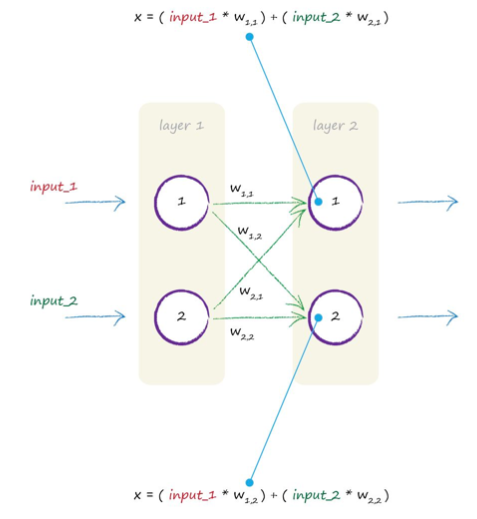
\includegraphics[width=0.7\linewidth]{images/TEMPSimpleNN}
		\end{figure}		

	\section{Uma rede neural simples}
		\par Como visto na figura \ref{fig:simpleNeuralNetwork} da sessão anterior uma rede neural conecta suas camadas usando pesos que servirão como moderadores das entradas da próxima camada com o fim desse evitar o \textit{overfitting}. É possível representar uma rede neural de várias formas, no entanto, como ilustrado na figura \ref{fig:matrixmultnn}, a forma mais eficiente computacionalmente será a matricial, usando esta abordagem será possível representar facilmente as camadas e os respectivos pesos que as ligam, melhorando também o desempenho computacional já que tais operações são altamente paralelizáveis.
		
		
		\begin{figure}[H]
			\centering
			\caption[Representação de uma rede neural usando matrizes]{Representação de uma rede neural usando matrizes}
			\label{fig:matrixmultnn}
			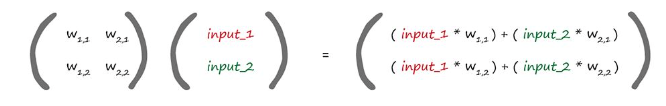
\includegraphics[width=0.7\linewidth]{images/TEMPMatrixMultNN}
		\end{figure}
		
	\section{Redes neurais multicamadas}
		\par A depender da complexidade do problema apenas duas camadas não são suficientes para que este aproximados universal de funções, mais conhecido como rede neural, consiga obter resultados satisfatórios. Assim, se torna necessário adição de uma ou mais camadas que servirão para aumentar a complexidade do espaço das soluções de nossa rede.
		
		\par Então, considerando o contexto, as tais camadas que devem ser adicionadas serão chamadas de ocultas ou \textit{hidden layers}\cite{rashid2016make}. 
		
		\par Em redes neurais multicamadas surge um novo problema: Como atualizar os valores dos pesos entre as camadas já que o erro produzido depende das várias entradas da camada anterior? Como mostrado na figura \ref{fig:simpleNeuralNetwork} o valor da próxima camada depende da soma ponderada pelos pesos dos valores da anterior sendo que tal soma deve passar por uma função de ativação escolhida, portanto, após o cálculo do erro na resposta da rede é preciso recalcular os pesos de forma a distribuir esses erros usando um algoritmo ao qual daremos o nome de retro-propagação ou \textit{backpropagation} \cite{haykinredes}. É importante frisar que este é apenas um dos vários métodos de treinamento da rede neural, é possível, por exemplo, usar uma abordagem bio-inspirada e/ou evolutiva.
		
		\begin{figure}[H]
			\centering
			\caption{Retro-propagação}
			\label{fig:backpropagation}
			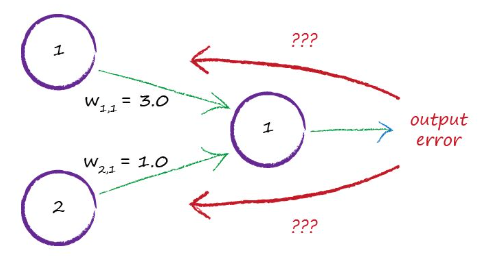
\includegraphics[width=0.7\linewidth]{images/TEMPbackpropagation}
		\end{figure}
	
	\section{Retro-propagação}
		\par Primeiramente é importante notar que os pesos associados a cada item da camada (neurônio) Contribuem com o erro resultante de forma proporcional aos seus respectivos valores, sendo assim, é necessário ao fazer a retro-propagação que esses erros sejam distribuídos proporcionalmente como indicado na figura \ref{fig:backpropagationErrors}.
		
		\begin{figure}[H]
			\centering
			\caption{Parcela da distribuição do erro na retro-propagação para o $erro_1$, o mesmo deve ser feito para todos os outros erros.}
			\label{fig:backpropagationErrors}
			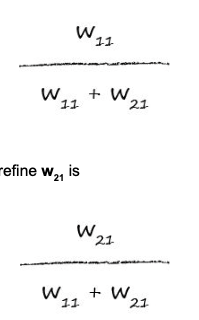
\includegraphics[width=0.4\linewidth]{images/TEMPbackpropagationErros}
		\end{figure}
		
		\par Calculada a parcela da participação de cada peso nos erros produzidos, Se passar a fase do erro resultante na camada oculta para que, usando o mesmo raciocínio de cálculo da participação no erro, se possa continuar com algoritmo de retro-propagação. Assim, o cálculo do erro da camada oculta se dar como mostrado na equação \ref{eq:hiddenLayerError}.
		
		\begin{equation}
			\label{eq:hiddenLayerError}
			erro_{oculto_1} = \begin{cases} 
				erro_{resultado_1}  * \dfrac{peso_{1,1}}{peso_{1,1} + peso_{2,1}+ ... + peso_{n,1}}  + \\\\
				erro_{resultado_2}  * \dfrac{peso_{1,2}}{peso_{1,2} + peso_{2,2}+ ... + peso_{n,2}}  + \\
				\qquad\qquad \vdots \\
				+ erro_{resultado_k}  * \dfrac{peso_{1,k}}{peso_{1,k} + peso_{2,k}+ ... + peso_{n,k}} 
			\end{cases}			 
		\end{equation}
	
		\par Onde, em relação ao neurônio atual da camada oculta($oculto_1$), $n$ representa a quantidade de pesos vinculados e $k$ o número de neurônios na camada de saída . As figuras \ref{fig:backpropagationerros1} e \ref{fig:backpropagationerros2} mostram em mais detalhes o funcionamento do algoritmo.
		
		\begin{figure}[H]
			\centering
			\caption{Retro-propagação da camada de saída para a oculta}
			\label{fig:backpropagationerros1}
			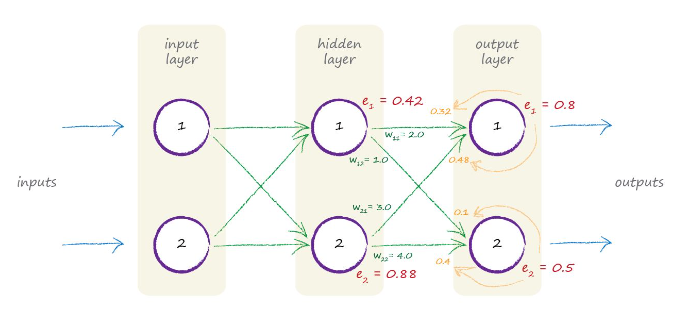
\includegraphics[width=0.7\linewidth]{images/TEMPbackpropagationErros1}
		\end{figure}
		
		
		\begin{figure}[H]
			\centering
			\caption{Retro-propagação da camada oculta para a entrada}
			\label{fig:backpropagationerros2}
			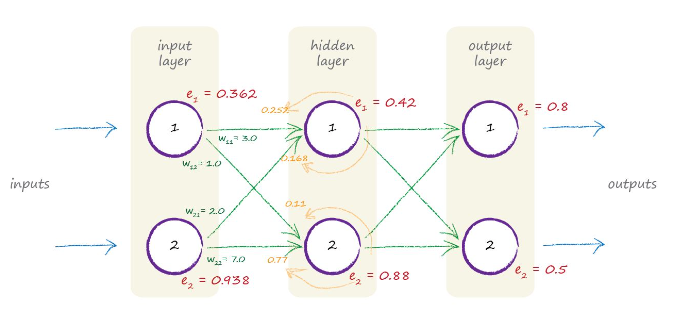
\includegraphics[width=0.7\linewidth]{images/TEMPbackpropagationErros2}
		\end{figure}
		
	\chapter{Paralelismo}
		\par 
		
		
\end{apendicesenv}









